L'avvento e la diffusione di Internet ha rivoluzionato il mondo in cui viviamo e reso possibile tra le altre cose anche una nuova concezzione di apprendimento. Nascono quindi i primi servizi di E-Learning che nel corso degli anni si sono evoluti e oggi giorno vengono comunemente chiamati anche MOOC(Massive Open Online Course).

La differenza sostanziale rispetto al passato sta nel fatto che le piattaforme MOOC offrono generalmente corsi aperti a chiunque, in cui la partecipazione è gratuita e permettono interattività tra gli studenti.
L'enorme potenziale di tali sistemi è stata compreso sin da subito e già nel 2012 tali servizi erano circa 100 e quasi 700 nel 2013, con una media di 2 nuovi MOOC al giorno.
Le piattaforme più diffuse al momento risultano essere Coursera, EdX, Udacity, Udemy e SkillShare.
La maggior parte di queste offrono corsi organizzati direttamente dagli atenei tra cui troviamo nomi prestigiosi come Stanford, Harvard, Berkeley, MIT. In generale i corsi ricoprono diverse tematiche e vengono erogati direttamente dai Professori degli atenei universitari.
Tutti i corsi sono gratuiti cavalcando la filosofia tipica dei MOOC, viene pero richiesto un compenso nel caso in cui si desideri ottenere una certificazione, rilasciata solo dopo aver superato un test per verificare il reale livello di apprendimento.

Questi sistemi sono stati accolti come una vera e propria rivoluzione nel mondo dell'istruzione, rendendo la formazione accessibile a chiunque eliminando barriere temporali e spaziali. Infatti la comodità e il vantaggio di queste piattaforme è poter seguire corsi universitari a migliaia di chilometri di distanza comodamente da casa e in qualsiasi momento e orario della giornata.

Nelle prime piattaforme di MOOC i corsi erano quindi tenuti dagli stessi docenti degli atenei, questo trend è pero cambiato negli ultimi anni e ha visto la nascita di nuove piattaforme in cui chiunque può creare un proprio corso.

Questa nuova opportunità offerta per esempio dal noto serivzio MOOC di Udemy, ha riscontrato subito un grande successo ed è stata sfruttata da molte persone che ne hanno fatto una vera e propria fonte di guadagno. 


\begin{figure}[htb] %  figure placement: here, top, bottom
 \centering
 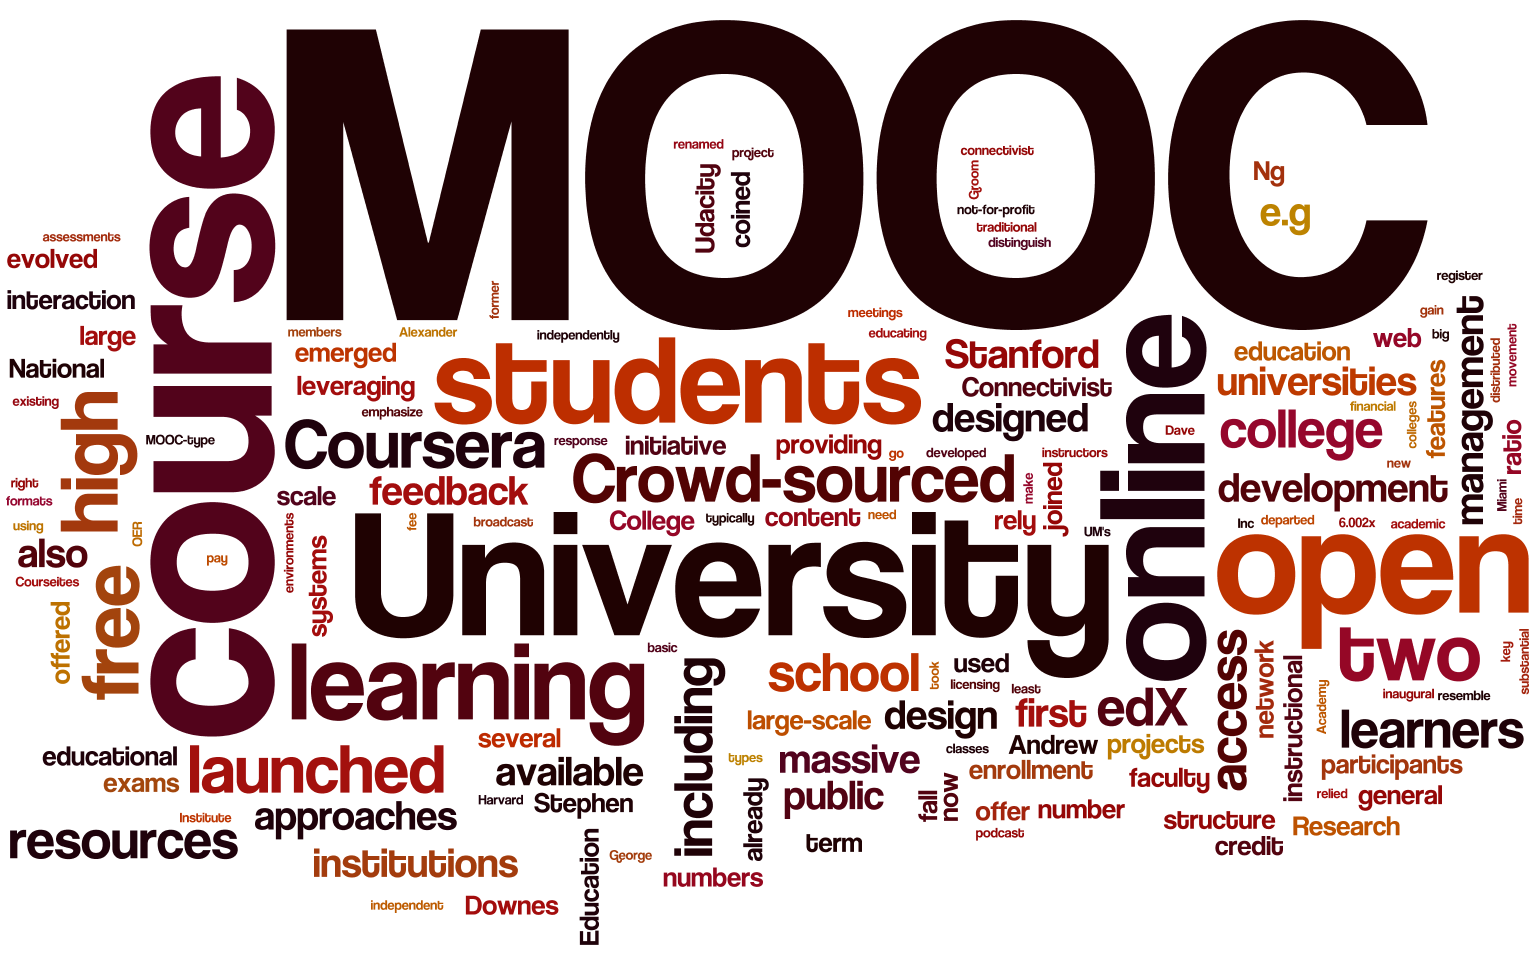
\includegraphics[width=0.8\linewidth]{images/introduction/mooc.png}\hfill
 \caption[Mooc image]{Mooc image}
 \label{fig:fourV}
\end{figure}

Creare un serizio di e-learning richiede tuttavia investimenti onerosi per coprire i costi di realizzazione, storage e soprattuto per il traffico dati necessario per lo streaming dei contenuti video.

Inoltre nonostante l'avvento di HTML5 la gestione video rimane ancora molto insidiosa, non esiste infatti un standard per lo streaming in grado di garantire la fruzione dei contenuti su i diversi web browser e dispositivi mobili.
E' evidente quindi come la creazione di una piattaforma di learning richieda necessarimante conoscenze tecniche e tecnologiche.


L'obietivo del mio progetto di tesi svolto presso il CVDLAB è quello di semplificare e nascodere tutti i problemi sopra elencati e quindi offrire l'opportunita a utenti e principalmente aziende di creare la propria piattaforma di E-Learning dove vengono offerti esclusivamente i loro corsi.

Inoltre nella fase finale del progetto ho potuto constatare personalmente come il concetto di riusabilità dei componenti preso in prestito dai Web Components abbia facilitato notevolmente la creazione di un caso d'uso: X-Learning.

Come vedremo nei capitoli successivi X-Learning puo essere diviso in due parti ben distinte composte rispettivamente da:
\begin{itemize}
\item Admin che puo inserire i corsi e invitare i collaboratori nella propria piattaforma,
\item Utente che può navigare la piattaforma e seguire i corsi desiderati
\end{itemize}
Il passo successivo come vedremo nel capitolo dei sviluppi futuri sarà proprio il deploy del servizio per renderlo utilizzabile a chiunque.

%%%%%

% Il mio contributo finale che rappresenta il core di tale progetto è stato la creazione di una piattaforma di E-learning come Udemy dove ogni utente può creare i propri corsi, il passo successivo sara poi come vedremo nel capitolo dei sviluppi futuri il deploy del mio servizio.

La mia tesi è stata divisa in due parti ognuna composta da 3 capitoli.
Nel primo capitolo viene offerta una panoramica sulle piattaforme MOOC già esistenti.
Il secondo capitolo invece descrive i servizi utilizzati per la realizzazione della piattaforma e un breve analisi dei costi.
Nel terzo capitolo invece vengono illustrate le tecnologie adottate per lo sviluppo.
Con l'inizio della seconda parte della tesi entriamo nel dettaglio del progetto, in particolar modo nel quarto capitolo avremo una panoramica della architettura e organizzazione della piattaforma.
Nel quinto capitolo ci focalizzeremo su componenti principali realizzati nel progetto e su come sono stati realizzati.
Il sesto e ultimo capitolo espone le conclusione tratte e fornisce dei possibili sviluppi futuri.
